\documentclass[11pt]{article}

\usepackage[letterpaper,top=0.45in,bottom=0.45in,left=0.50in,right=0.50in]{geometry}
\usepackage[T1]{fontenc}
\usepackage{newtxtext,newtxmath}
\usepackage{microtype}

\usepackage{xcolor}
\usepackage{titlesec}
\usepackage{tikz}
\usepackage[hidelinks]{hyperref}
\usetikzlibrary{arrows.meta,positioning,calc}

\definecolor{accent}{RGB}{30,72,120}
\definecolor{soft}{RGB}{245,247,250}
\setlength{\parindent}{0pt}
\setlength{\parskip}{2.5pt}
\AtBeginDocument{\fontsize{11}{12.8}\selectfont}
\pagestyle{empty}
\titleformat{\section}{\bfseries\color{accent}\normalsize}{}{0pt}{}
\titlespacing*{\section}{0pt}{5pt}{1.5pt}

% ===== Author/title fields =====
\newcommand{\projecttitle}{AgentQEC: Learning to Coordinate Agents for Efficient\\Quantum Error-Correcting Code Discovery}
\newcommand{\studentA}{Shubdeep Mohapatra}
\newcommand{\studentB}{Yongxiang Lyu}
\newcommand{\university}{North Carolina State University}

\begin{document}
\begingroup\centering
    {\Large\bfseries \projecttitle}\\[2pt]
    {\small \studentA\textsuperscript{1}\qquad \studentB\textsuperscript{1}}\\[1pt]
    {\small \textsuperscript{1}\,\university}
\par\endgroup
\vspace{2pt}

\section*{Motivation and Problem}
Quantum computing changes the scaling of selected computations: Shor's algorithm factors integers in polynomial time, whereas no polynomial-time classical algorithm is known~\cite{shor}. Unlike the reliable-gate abstraction of classical computing, physical quantum operations remain error-prone: entangling-gate infidelities near $10^{-3}$ have been reported, while many applications target logical error rates below $10^{-10}$~\cite{googleqec}. \textbf{Quantum error correction (QEC)} addresses this gap by encoding logical information across multiple physical qubits. A \emph{QEC code} specifies the encoding and error checks that reveal faults without reading out the protected quantum state.

QEC discovery balances reliability, qubit overhead, and hardware constraints. Experts construct algebraic code families, while heuristic and reinforcement-learning methods explore candidate codes and encoding circuits~\cite{olle}. We ask: \textbf{how should an AI system allocate reasoning, communication, and evaluation resources as evidence about a candidate changes?} Algebraic checks can be inexpensive and exact, whereas decoding and noise simulations provide costly statistical estimates. Fixed agent workflows cannot adapt this allocation.

\section*{Proposed Innovation: Learning to Coordinate}
We propose \textbf{AgentQEC}, a multi-agent system with \textbf{evidence-conditioned, budget-aware coordination}. Designer and critic agents propose and refine codes; executable mathematical checkers and numerical simulators test them. Building on cost-aware agent coordination~\cite{corl}, we will learn a controller that jointly selects the next specialist, its inference budget, and the fidelity of tool evaluation. Decisions depend on candidate structure, verification history, evaluation uncertainty, remaining budget, and measured runtime state---not a predetermined sequence of agent calls.

\textbf{Learning from heterogeneous feedback.} We will train the controller with cost-constrained reinforcement learning on tool-annotated search trajectories, initially keeping specialist models fixed. Exact validity violations, estimated code properties, and confidence intervals on logical-error rates remain distinct in the state representation. Intermediate results guide repair and evaluation decisions; high-fidelity assessments supply the final quality signal. A failed commutation check triggers repair rather than simulation, while uncertain performance can justify additional samples. The controller must learn when stronger evidence justifies its cost, without treating cheap proxies as verified improvements.

\vspace{2pt}
\begingroup\centering
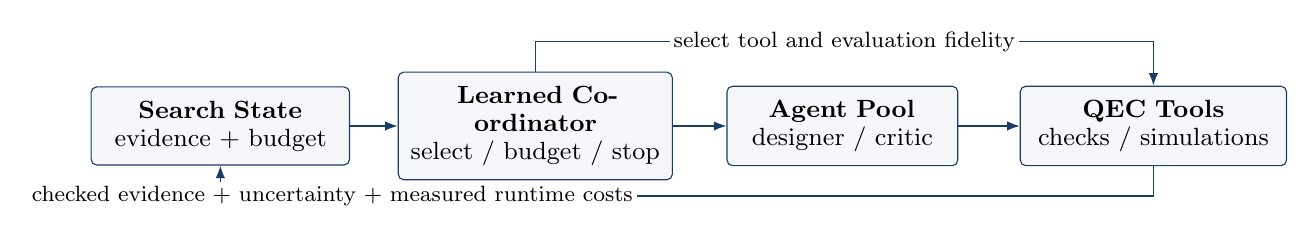
\begin{tikzpicture}[
    font=\fontsize{9}{10.2}\selectfont,
    box/.style={draw=accent!85!black,rounded corners=2pt,fill=soft,
        inner xsep=4pt,inner ysep=5pt,align=center,minimum height=0.70cm},
    arrow/.style={-{Latex[length=1.6mm]},line width=0.5pt,draw=accent!85!black},
    lab/.style={font=\fontsize{8.1}{9}\selectfont,fill=white,inner sep=1.5pt}
]
\node[box,text width=3.0cm] (state) at (0,0) {\textbf{Search State}\\evidence + budget};
\node[box,text width=3.2cm] (coord) at (4.0,0) {\textbf{Learned Coordinator}\\select / budget / stop};
\node[box,text width=2.65cm] (agents) at (7.9,0) {\textbf{Agent Pool}\\designer / critic};
\node[box,text width=3.1cm] (tools) at (11.85,0) {\textbf{QEC Tools}\\checks / simulations};
\draw[arrow] (state.east) -- (coord.west);
\draw[arrow] (coord.east) -- (agents.west);
\draw[arrow] (agents.east) -- (tools.west);
\draw[arrow] (coord.north) -- ++(0,0.38) -| node[pos=0.25,lab] {select tool and evaluation fidelity} (tools.north);
\draw[arrow] (tools.south) -- ++(0,-0.38) -| node[pos=0.44,lab] {checked evidence + uncertainty + measured runtime costs} (state.south);
\end{tikzpicture}\par\endgroup
\vspace{1pt}

\section*{Agentic System Efficiency and QEC Quality}
\textbf{Agentic system efficiency} targets avoidable inference, inter-agent communication, and synchronization overhead. The controller selectively activates specialists and budgets their context exchange. Shared structured records reuse tool results only when candidate, noise, and decoder settings match; dependency-aware scheduling overlaps independent checks and reasoning. We will measure latency, GPU time, peak memory, tokens, communication volume, and tool time, including coordination overhead; training costs will be reported separately. \textbf{QEC system efficiency} is evaluated through logical-error rate at fixed noise and decoder settings, physical-qubit overhead, syndrome-extraction depth, and decoder latency. We will compare agent cost at matched QEC quality and QEC quality at matched budgets, rather than assume simultaneous gains in both.

\section*{One-Year Scope and Evaluation}
Year one will deliver a CSS-code prototype, learned controller, and reproducible benchmark. On held-out noise settings and code sizes, we will compare fixed, rule-based, and learned coordination using the same specialist/tool pool, alongside single-agent and heuristic/RL code-search baselines. Ablations will isolate feedback, routing, and shared-state scheduling to quantify the quality--compute tradeoff.

% Compact, self-contained references: no BibTeX step or external .bib is needed.
% These support background claims, not a claim of first-ever learned orchestration.
\begingroup
\renewcommand{\section}[2]{}%
\fontsize{8.1}{9.2}\selectfont
\setlength{\parskip}{0pt}
\begin{thebibliography}{4}
\setlength{\itemsep}{0pt}\setlength{\parsep}{0pt}
\bibitem{shor} P.~W.~Shor. \href{https://arxiv.org/abs/quant-ph/9508027}{Polynomial-Time Algorithms for Prime Factorization and Discrete Logarithms on a Quantum Computer}. \emph{SIAM J. Comput.} 26, 1484--1509 (1997).
\bibitem{googleqec} Google Quantum AI and Collaborators. \href{https://doi.org/10.1038/s41586-024-08449-y}{Quantum error correction below the surface code threshold}. \emph{Nature} 638, 920--926 (2025).
\bibitem{olle} J.~Olle et al. \href{https://arxiv.org/abs/2311.04750}{Simultaneous discovery of quantum error correction codes and encoders with a noise-aware reinforcement learning agent}. arXiv:2311.04750 (2023).
\bibitem{corl} B.~Jin et al. \href{https://arxiv.org/abs/2511.02755}{Controlling Performance and Budget of a Centralized Multi-agent LLM System with Reinforcement Learning}. arXiv:2511.02755 (2025).
\end{thebibliography}
\endgroup
\end{document}
